\chapter{Interprétabilité du modèle final}

Après la sélection et l'évaluation du modèle final, l'analyse ne s'arrête pas aux métriques. Il est nécessaire de comprendre quelles variables influencent les prédictions et si ces variables ont une signification physique cohérente. Le modèle retenu étant un ensemble d'arbres, trois approches complémentaires sont utilisées : l'importance native des variables, les valeurs SHAP et la permutation importance.

\section{Importance native des variables}

L'importance native des variables mesure la contribution moyenne de chaque variable dans les divisions des arbres. Elle fournit une première lecture rapide du comportement du modèle. Cette méthode doit cependant être interprétée avec prudence, car elle peut être influencée par les corrélations entre variables.

\begin{figure}[htbp]
    \centering
    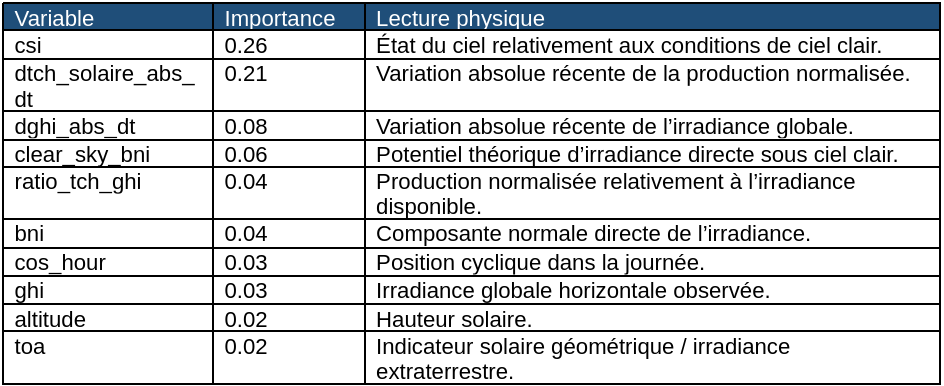
\includegraphics[width=0.7\textwidth]{img/tab_7_1.png}
    \caption{Dix premières variables selon l'importance native du modèle ExtraTrees.}
    \label{fig:tab_7_1}
\end{figure}

\begin{figure}[htbp]
    \centering
    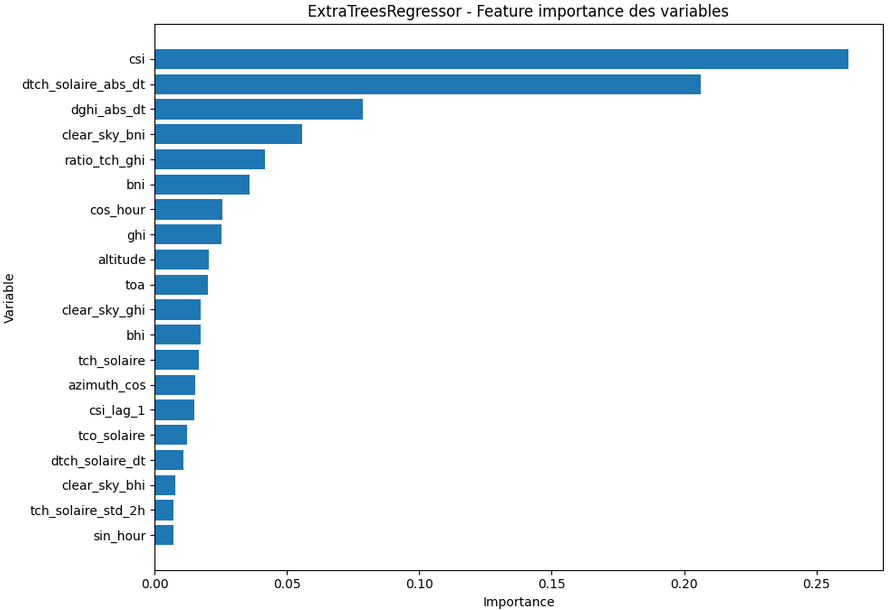
\includegraphics[width=0.7\textwidth]{img/var_nat_imp.png}
    \caption{Importance native des vingt premières variables du modèle ExtraTrees.}
    \label{fig:var_nat_imp}
\end{figure}

Les variables les plus importantes sont \textit{csi}, \textit{dtch\_solaire\_abs\_dt}, \textit{dghi\_abs\_dt} et \textit{clear\_sky\_bni}. Le modèle utilise donc principalement l'état du ciel par rapport au ciel clair, l'instabilité récente de la production, la variation récente de l'irradiance globale et le potentiel théorique d'irradiance directe par ciel clair.

Ce résultat est physiquement cohérent : la variabilité photovoltaïque à court terme dépend fortement de l'état atmosphérique, des changements récents d'irradiance et de la capacité du moment étudié à produire une variation visible de production.

\section{Analyse SHAP}

L'analyse SHAP apporte une interprétation plus détaillée que l'importance native. Elle estime, pour chaque observation, la contribution de chaque variable à la prédiction du modèle. Une valeur SHAP positive augmente la variabilité photovoltaïque prédite, tandis qu'une valeur SHAP négative la diminue.


\begin{figure}[htbp]
    \centering
    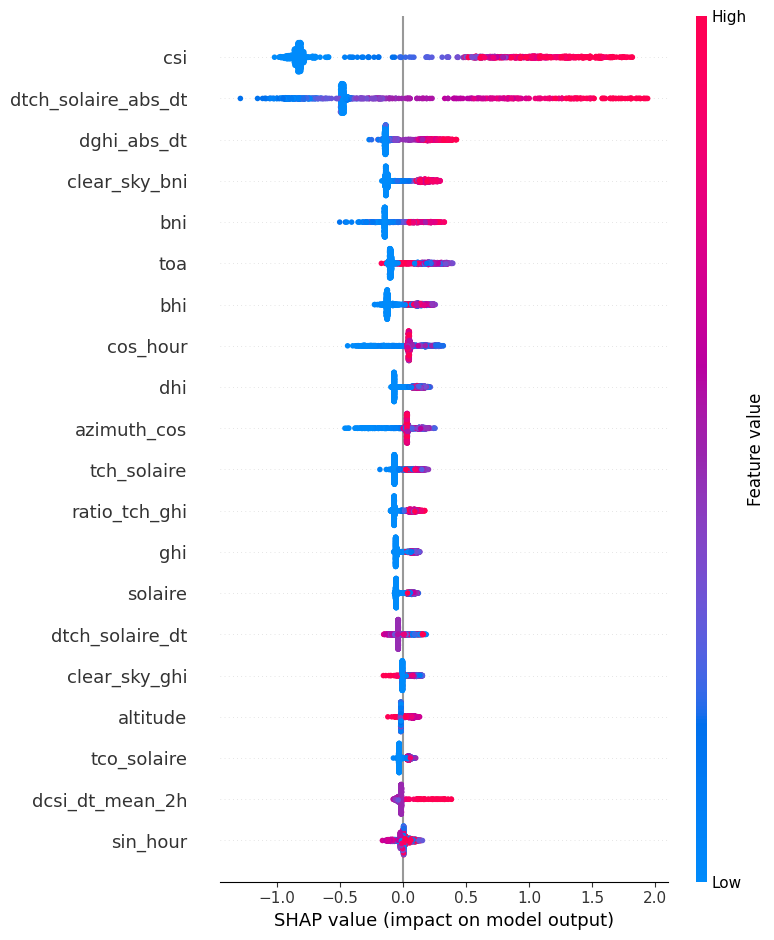
\includegraphics[height=0.5\textheight]{img/shap.png}
    \caption{Résumé SHAP : effet des variables sur les prédictions.}
    \label{fig:shap}
\end{figure}

Les résultats SHAP confirment que le modèle apprend principalement trois types d'information : l'état du ciel par rapport au ciel clair, l'instabilité récente de la production solaire normalisée et les variations récentes de l'irradiance. Les variables les plus influentes sont notamment \textit{csi}, \textit{dtch\_solaire\_abs\_dt}, \textit{clear\_sky\_bni} et \textit{dghi\_abs\_dt}.

Le \textit{csi} indique si le rayonnement observé est proche des conditions de ciel clair. Lorsqu'il est élevé, le potentiel de production est important et une perturbation atmosphérique peut entraîner une variation plus visible de la production. De même, \textit{clear\_sky\_bni} apporte un contexte physique sur le potentiel de rayonnement direct disponible selon la position du soleil, ce qui aide le modèle à identifier les périodes où une forte variation est possible.

La variable \textit{dtch\_solaire\_abs\_dt} mesure l'instabilité récente de la production. Lorsqu'elle est élevée, elle pousse généralement la prédiction vers une variabilité future plus importante, ce qui est cohérent avec l'idée qu'un système déjà instable peut rester instable à court terme. Enfin, \textit{dghi\_abs\_dt} et les autres variables radiatives, comme \textit{GHI}, \textit{DHI} ou \textit{BNI}, permettent d'identifier les changements rapides de conditions lumineuses, souvent liés aux passages nuageux.

Ainsi, les variables de ciel clair, les variables radiatives et les encodages temporels donnent au modèle un contexte physique supplémentaire : elles indiquent si la situation correspond à un moment de fort potentiel solaire, à une transition matin/soir ou à une anomalie atmosphérique. Comme la cible est une différence absolue, le modèle prédit l'intensité de la variation future, mais pas son sens.

\section{Permutation importance}

La permutation importance mesure l'importance d'une variable en observant l'augmentation de l'erreur lorsque ses valeurs sont mélangées aléatoirement. Contrairement à l'importance native des arbres, elle évalue directement l'utilité de la variable pour la performance prédictive du modèle final.

Dans le notebook, cette analyse est appliquée sur l'ensemble de test. Ce choix est important, car il permet d'interpréter l'importance des variables sur des données non utilisées pendant l'entraînement ni pendant l'optimisation du modèle.


\begin{figure}[htbp]
    \centering
    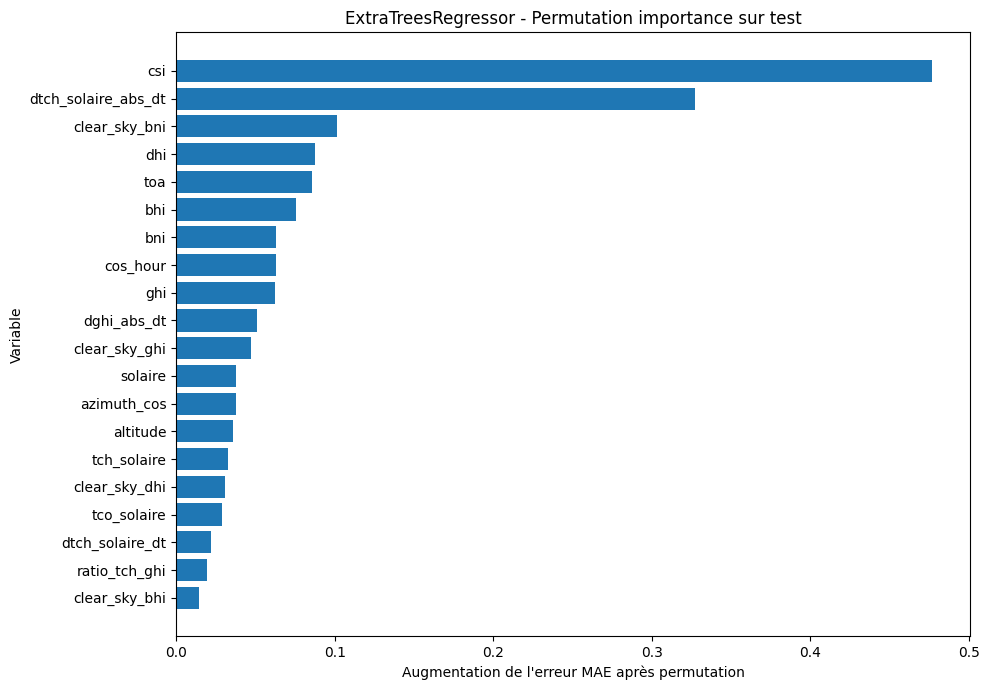
\includegraphics[width=0.8\textwidth]{img/var_imp.png}
    \caption{Permutation importance du modèle ExtraTrees sur l'ensemble de test.}
    \label{fig:var_imp}
\end{figure}

La permutation importance confirme les résultats précédents. Les variables \textit{csi} et \textit{dtch\_solaire\_abs\_dt} dominent clairement l'interprétation, avec des augmentations moyennes de MAE d'environ 0.37 et 0.32 après permutation.

La présence de \textit{clear\_sky\_bni} en troisième position est particulièrement importante. Elle montre que le modèle ne dépend pas uniquement des variations observées dans le passé, mais aussi du contexte physique de ciel clair et du potentiel de rayonnement direct. Autrement dit, le modèle apprend qu'une même perturbation atmosphérique n'a pas le même impact selon le niveau de rayonnement direct théoriquement disponible.

Les autres variables importantes, comme \textit{ghi}, \textit{bni}, \textit{dghi\_abs\_dt}, \textit{bhi}, \textit{clear\_sky\_ghi} et \textit{dhi}, confirment que les variations de production photovoltaïque sont fortement liées aux niveaux d'irradiance et aux changements rapides des conditions lumineuses. L'accord entre feature importance, SHAP et permutation importance renforce la confiance dans le modèle, car les variables dominantes ont un sens physique clair.
